This section gives the PIE analogue of the finite-dimensional overview in the preceding
section. The central point is that the primal-dual construction can be written directly
in terms of PI operators: the primal scaling defines a scaled input-output map, the
adjoint PIE defines the dual dynamics, and the dual scaling is determined algebraically
from the primal scaling.

\begin{definition}\label{def:primalscaledsys}
    For $w(t)\in\RL^{\mbf{n}_w}$, $\mbf{x}(t)\in\RL^{\mbf{n}_\mbf{x}}$, and
    $z(t)\in\RL^{\mbf{n}_z}$ that satisfy $\mbf{x}(0) = 0$, the \textbf{Primal System}
    $G\{\mcl{T}, \mcl{A}, \mcl{B}, \mcl{C}, \mcl{D}\}$ is defined as,
    \begin{equation}\label{eqn:primalsys}
        \bmat{\mcl{T}\dot{\mbf{x}}(t)\\ z(t)} = \bmat{\mcl{A} & \mcl{B} \\
        \mcl{C} & \mcl{D}}\bmat{\mbf{x}(t) \\ w(t)}
    \end{equation}
    where $\mcl{T}, \mcl{A}\in \Pi_4^{\mbf{n}_\mbf{x} \times \mbf{n}_\mbf{x}}$,
    $\mcl{B}\in\Pi_4^{\mbf{n}_w \times \mbf{n}_\mbf{x}}$,
    $\mcl{C}\in\Pi_4^{\mbf{n}_\mbf{x}\times\mbf{n}_z}$, and
    $\mcl{D}\in\Pi_4^{\mbf{n}_w \times \mbf{n}_z}$ are PI operators.
    The \textbf{Scaled Primal System} is expressed in terms of $\tilde{w}(t)\in
    \RL^{\mbf{n}_w}$ and $\tilde{z}(t)\in\RL^{\mbf{n}_z}$, which satisfy,
    \begin{equation}\label{eqn:primalscaling}
        \bmat{z(t) \\ w(t)} = \underbrace{\bmat{\mcl{S}_{11} & \mcl{S}_{12} \\
        \mcl{S}_{21} & \mcl{S}_{22}}}_{\mcl{S}}\bmat{\tilde{z}(t) \\ \tilde{w}(t)}.
    \end{equation}
    The operator $\mcl{S}$ is called the \textbf{Primal I/O Scaling} of the system.
\end{definition}


\begin{definition}\label{def:dualscaledsys}
    For $\underline{w}(t)\in\RL^{\mbf{n}_z}$, $\underline{\mbf{x}}(t)\in\RL^{\mbf{n}_\mbf{x}}$, and
    $\underline{z}(t)\in\RL^{\mbf{n}_w}$ that satisfy $\underline{\mbf{x}}(0) = 0$, the \textbf{Dual
    System} $\underline{G}\{\underline{\mcl{T}}, \underline{\mcl{A}}, \underline{\mcl{B}}, \underline{\mcl{C}},
    \underline{\mcl{D}}\} = G\{\mcl{T}^*, \mcl{A}^*, \mcl{C}^*, \mcl{B}^*, \mcl{D}^*\}$ is
    defined as,
    \begin{equation}\label{eqn:dualsys}
        \bmat{\mcl{T}^*\dot{\underline{\mbf{x}}}(t)\\ \underline{z}(t)} = \bmat{\mcl{A}^* &
        \mcl{C}^* \\ \mcl{B}^* & \mcl{D}^*}\bmat{\underline{\mbf{x}}(t) \\ \underline{w}(t)}.
    \end{equation}
    The \textbf{Scaled Dual System} is expressed in terms of $\tilde{\underline{w}}(t)\in
    \RL^{\mbf{n}_z}$ and $\tilde{\underline{z}}(t)\in\RL^{\mbf{n}_w}$, which satisfy,
    \begin{equation}\label{eqn:dualscaling}
        \bmat{\underline{z}(t) \\ \underline{w}(t)} = \underbrace{\bmat{\mcl{S}_{22}^* &
        -\mcl{S}^*_{12} \\ -\mcl{S}^*_{21} & \mcl{S}^*_{11}}^{-1}}_{\underline{\mcl{S}}}
        \bmat{\tilde{\underline{z}}(t) \\ \tilde{\underline{w}}(t)}.
    \end{equation}
    The operator $\underline{\mcl{S}}$ is called the \textbf{Dual I/O Scaling} of the system
    and is parameterized by entries from the \textbf{Primal I/O Scaling}.
\end{definition}

\begin{theorem}[Scaled IO duality]\label{thm:dualscaledIO}
Assume the following conditions hold
\begin{itemize}
    \item The \textbf{Primal I/O Scaling} is a PI operator and invertible.
    \item $\mcl{S}_{11} - \mcl{D}\mcl{S}_{21}$ and $\underline{\mcl{S}}_{11} - \mcl{D}^*\underline{\mcl{S}}_{21}$ are invertible.
\end{itemize}
    The following statements are equivalent.
    \begin{enumerate}
    \item For all $\tilde{w}\in\RL^{\mbf{n}_w}$, the \textbf{Scaled Primal System}
    satisfies $\|P_\tau\tilde{z}\| \leq \|P_\tau\tilde{w}\|$.
    \item For all $\tilde{\underline{w}}\in\RL^{\mbf{n}_z}$, the \textbf{Scaled Dual System}
    satisfies $\|P_\tau\tilde{\underline{z}}\| \leq \|P_\tau\tilde{\underline{w}}\|$.
\end{enumerate}
\end{theorem}

The PIE generalized plant used in the IQC construction is
\begin{equation}\label{eqn:pie_gp}
    \begin{aligned}
        \mcl{T}\dot{\mbf{x}}_f(t)
        &=
        \mcl{A}\mbf{x}_f(t)
        +\mcl{B}_\Delta w_\Delta(t)
        +\mcl{B}_w w(t),\\
        z_\Delta(t)
        &=
        \mcl{C}_\Delta\mbf{x}_f(t)
        +\mcl{D}_\Delta w_\Delta(t)
        +\mcl{D}_{\Delta w}w(t),\\
        z(t)
        &=
        \mcl{C}_z\mbf{x}_f(t)
        +\mcl{D}_{z\Delta}w_\Delta(t)
        +\mcl{D}_{zw}w(t).
    \end{aligned}
\end{equation}
The uncertainty IQC is imposed on the filtered signal
\begin{equation}\label{eqn:pie_unc_iqc}
    v(t)
    =
    \Psi\bmat{z_\Delta(t)\\w_\Delta(t)},
    \qquad
    \ip{p_T v}{p_T\mcl{M}_{\mcl{V}_\Delta}v}_{\mbf{L}_{[a,b]}}
    \geq 0.
\end{equation}

The filter $\Psi$ is often tall rather than square
\cite{koserobust,veenman2016robust}. To obtain an invertible coordinate
transform, we complete it to a square filter. More generally, the completion is described by a projection from the square
coordinates back to the original IQC coordinates and by a right inverse of that
projection. Thus we choose operators $\mcl{N}_v$ and $\mcl{E}_v$ satisfying
\begin{equation}\label{eqn:pie_selector}
    v=\mcl{N}_v v_\square,
    \qquad
    \mcl{N}_v\mcl{E}_v=I.
\end{equation}
The special choice $\mcl{E}=\mcl{N}^*$ corresponds to orthogonal
zero-completion, but the construction does not rely on that choice. The IQC in
the square coordinates is defined using a freely chosen square-coordinate
multiplier $\mcl{M}_{\mcl{V}_\Delta}^{\square}$:
\begin{equation}
    \ip{p_T v_\square}
    {p_T\mcl{M}_{\mcl{V}_\Delta}v_\square}_{\mbf{L}_{[a,b]}}
    \geq 0,
\end{equation}
where $\mcl{M}_{\mcl{V}_\Delta}$ is selected directly in the
completed coordinates.

What needs to be done before applying Theorem~\ref{thm:dualscaledIO} in case we want to use dynamic multipliers,
\begin{enumerate}
    \item Start with the generalized PIE plant \eqref{eqn:pie_gp} and the dynamic IQC
    filter $\Psi$ in \eqref{eqn:pie_unc_iqc}. At this point the uncertainty is
    described in the original filtered coordinates $v$.

    \item Square up the filter. The projection $\mcl{N}$
    records which part of the square signal $v_\square$ enters the original IQC,
    while $\mcl{E}$ records how original coordinates are embedded into the
    square coordinates.

    \item Augment the generalized plant with the squared-up filter realization.
    If the uncertainty channel itself is also completed, use the same idea:
    project square inputs back to the original channel with a map $\mcl{N}$ and
    embed original outputs with a right inverse $\mcl{E}$ satisfying
    $\mcl{N}\mcl{E}=I$. The corresponding signal route is
    \[
        w_{\Delta,\square}
        \xrightarrow{\mcl{N}}
        w_{\Delta}
        \xrightarrow{G}
        z_{\Delta}
        \xrightarrow{\mcl{E}}
        z_{\Delta,\square}
        \xrightarrow{\Psi_\square}
        v_\square .
    \]
    If $\mcl{N}$ or $\mcl{E}$ is dynamic, its state is included in the augmented
    realization; the algebraic loop only sees the corresponding feedthrough
    operators.

    \item Close the resulting algebraic loop by the corresponding congruence
    transformation. This is the coordinate-free way of obtaining the scaled
    input-output map; a realization-level variable exchange is only one
    interpretation of the same substitution.

    \item Factor the chosen static PI multiplier as
    $\mcl{V}_\Delta=(\mcl{S})^*J\mcl{S}$, when such an
    invertible factorization is available. The congruence-closed realization
    gives the scaled primal input-output map used in
    Theorem~\ref{thm:dualscaledIO}.
\end{enumerate}

Apply Theorem~\ref{thm:dualscaledIO}. The 'adjoint' PIE gives the dual dynamics, and \eqref{eqn:dualscaling} gives the dual scaling
$\underline{\mcl{S}}$ from the primal scaling $\mcl{S}$. The resulting lower-right
    system is the scaled dual input-output map used for synthesis after constructing the dual multiplier 
    $\mathbf{D}(\mcl{V}) = \underline{\mcl{S}}^{-*}J\underline{\mcl{S}}^{-1}$, with the same bound as the scaled primal system.
    Figure~\ref{fig:pie-scaled-duality} summarizes the PIE duality construction according to Theorem~\ref{thm:dualscaledIO}. 
\begin{figure}[ht]
    \centering
    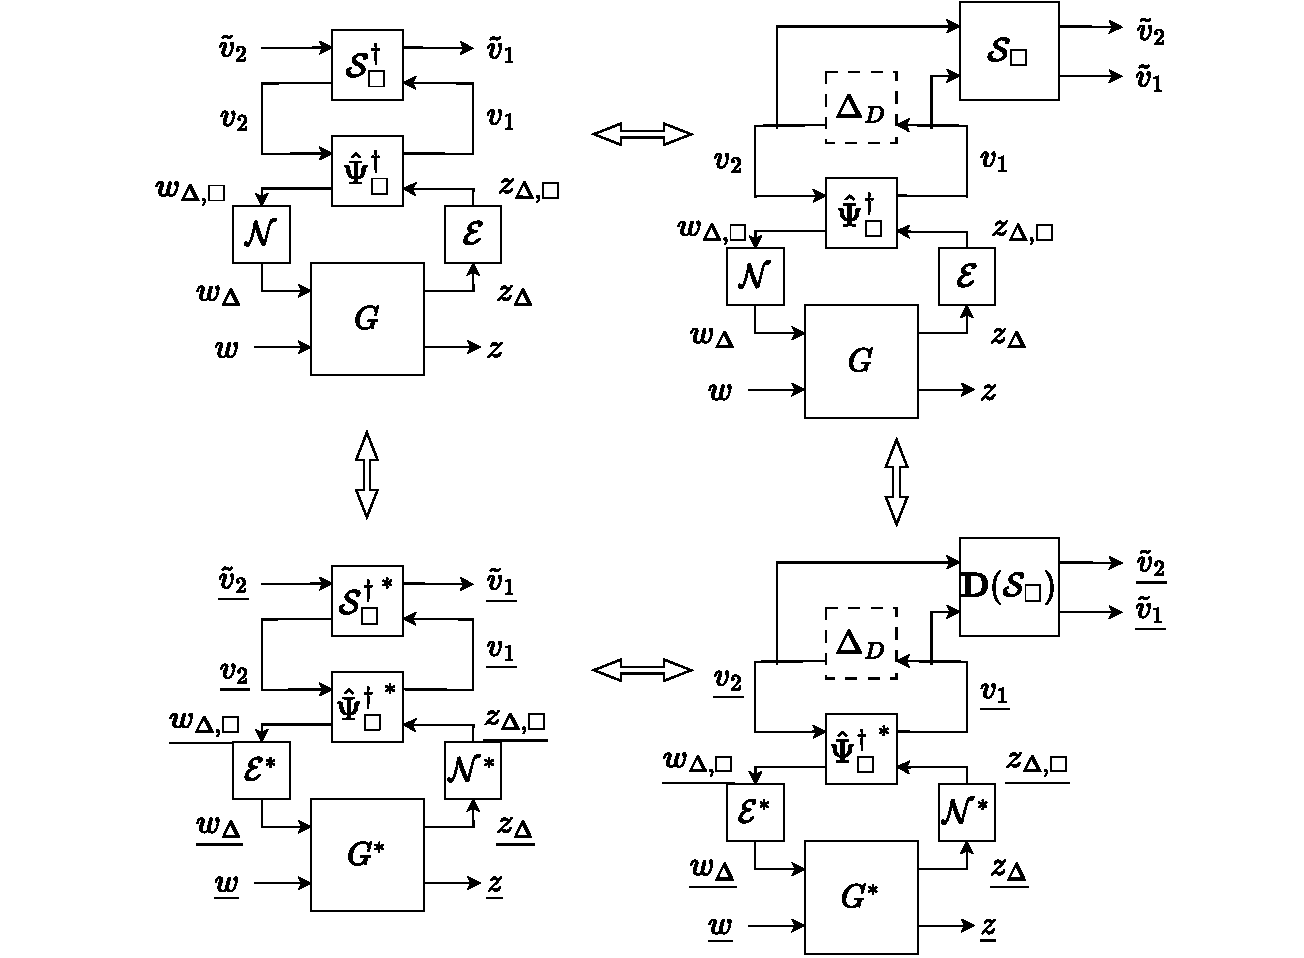
\includegraphics[width=0.8\textwidth]{Figures/Lenssen.pdf}
    \caption{Primal-dual correspondence for scaled PIE systems, adapted from
    \cite{lenssen2025muanalysissynthesisframeworkpartial}. The primal scaling induces
    the dual scaling, so both scaled systems represent equivalent input-output gain
    conditions.}
    \label{fig:pie-scaled-duality}
\end{figure}
